\documentclass{article}
\usepackage{amsmath}
\usepackage{amssymb}
\usepackage{graphicx}
\usepackage{hyperref}
\usepackage[version=4]{mhchem}

\title{Problem 8}
\date{}

\begin{document}
\maketitle

\section*{Problem}
\(\triangle A B C\) is a right triangle with \(\angle B A C=90^{\circ}\). The altitude to \(C B\) is draw from the vertex \(A\) to meet \(B C\) at \(F . D\) is a point on \(A C\) such that \(B D=D C=F C=6 \sqrt[3]{2}\). What is the length of \(A C\) ?\\
(A) \(\sqrt{2}\)\\
(B) \(\sqrt{3}\)\\
(C) 6\\
(D) \(\sqrt[3]{4}\)\\
(E) \(\sqrt[4]{2}\).\\
\centering
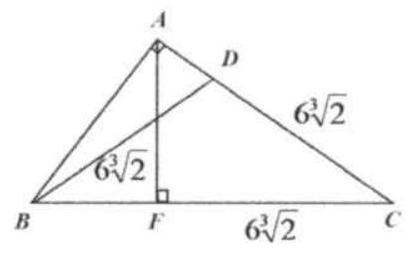
\includegraphics[width=\textwidth]{images/089(2).jpg}

\section*{Solution}
Solution not available.

\end{document}
